\subsection{Genotype Size \& Genotype mutations}

Figure~\ref{fig:Size} shows genotype size under the various studied conditions. The size is bounded (50 is the maximum size) and this limits differences between those environments as most simulations converge towards this limit, however, one can clearly see here that Short-cycle Fluctuation restrict the size of the genotypes while other forms of fluctuations do not appear to have any effect on genotype size. This size reduction could be a way to increase the impact of genotypic mutations on the phenotype. Indeed even if in LGP, when a mutation occurs its effect is proportional to the size of the genotype, long genotype may enable redundancy information to stabilize the phenotype. Figure~\ref{fig:Size} depicts the amount of mutations separating the current most common individual from individuals created at initialization of the simulation. It is not surprising that more mutations are selected when there are environmental fluctuations\footnote{And those seem to depend more on the strength of these fluctuations than on their periodicity.}, we note that the proximity of strong fluctuations and Short Cycle fluctuations indicates that their size differences is not explained by differences in the number of selected mutations.


\begin{figure}[h]
\centering
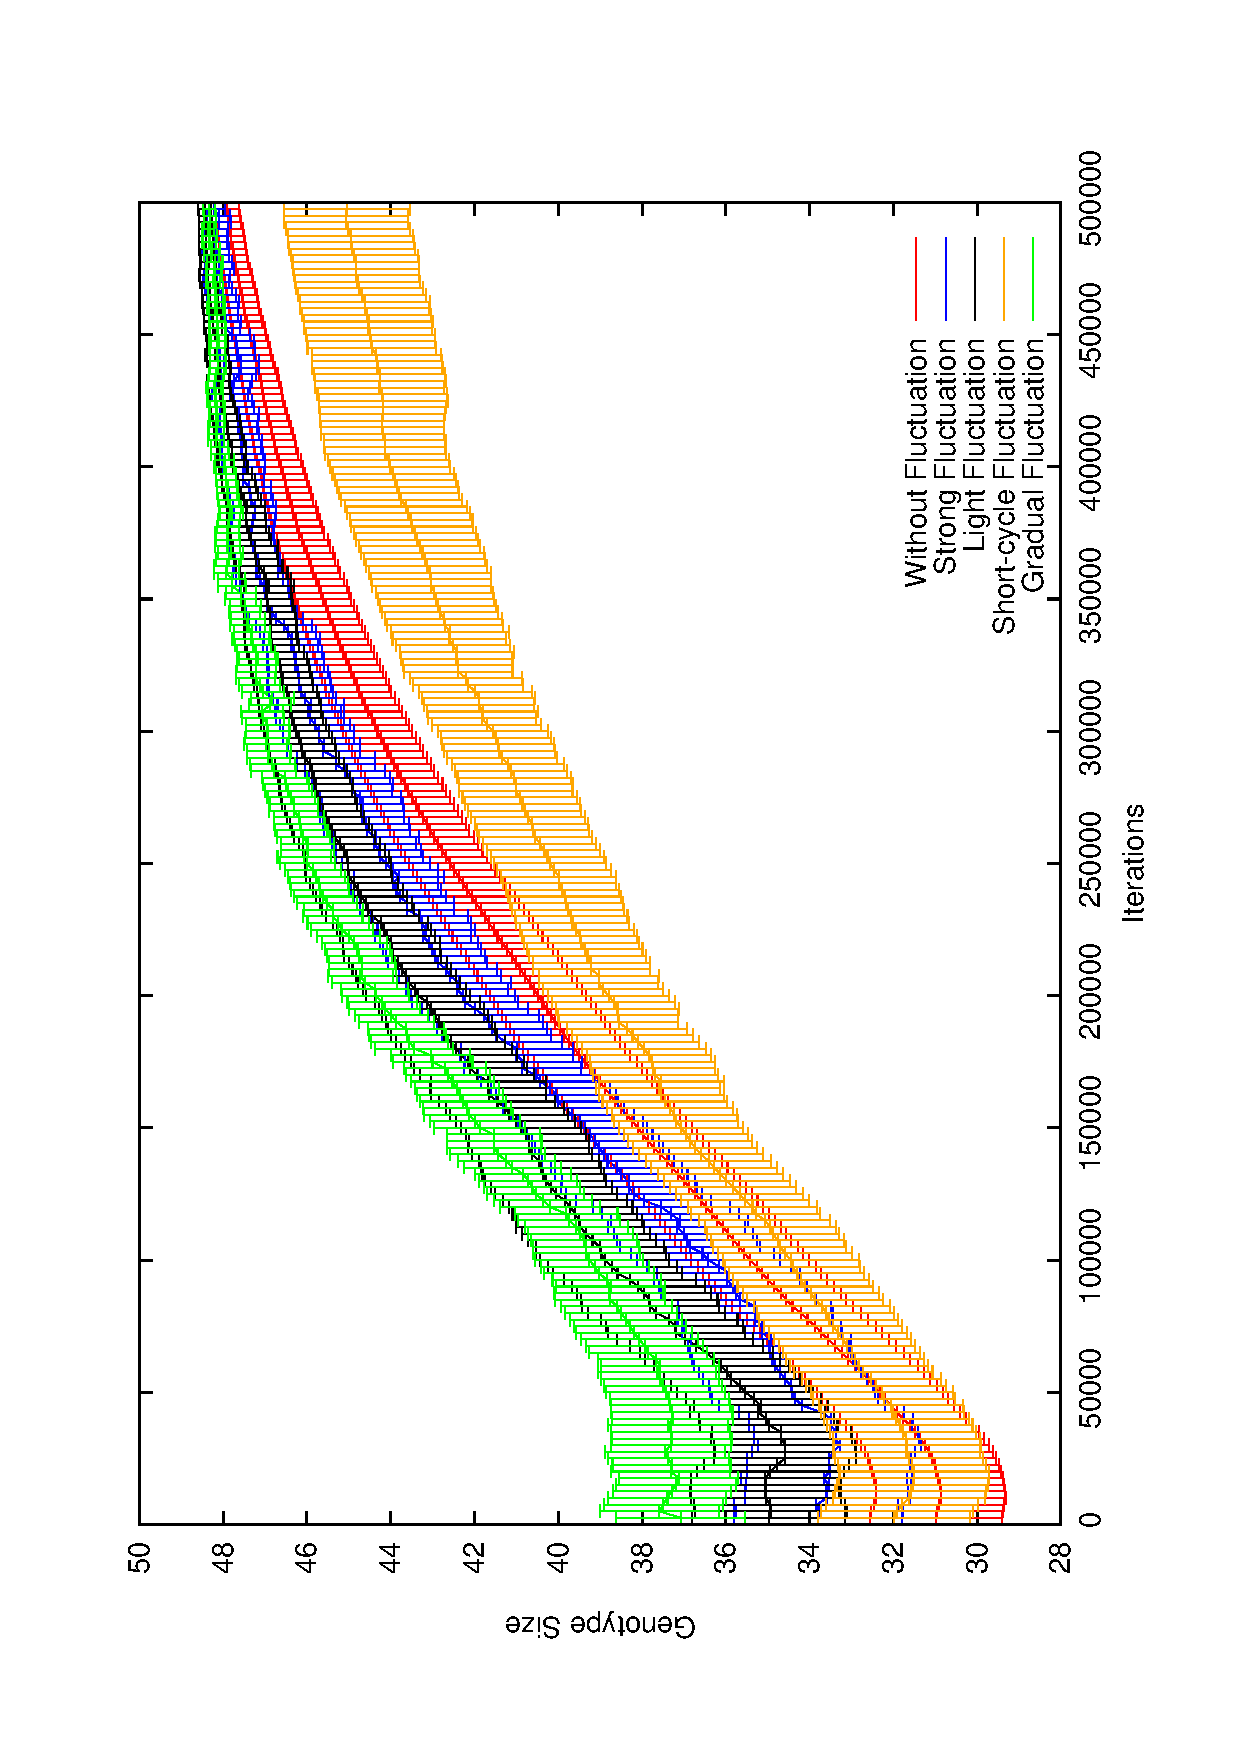
\includegraphics[width=0.7\columnwidth, angle =-90 ]{img/Size}
\caption{\textbf{Size of genotypes}. 
}
\label{fig:Size}
\end{figure}

\begin{figure}[h]
\centering
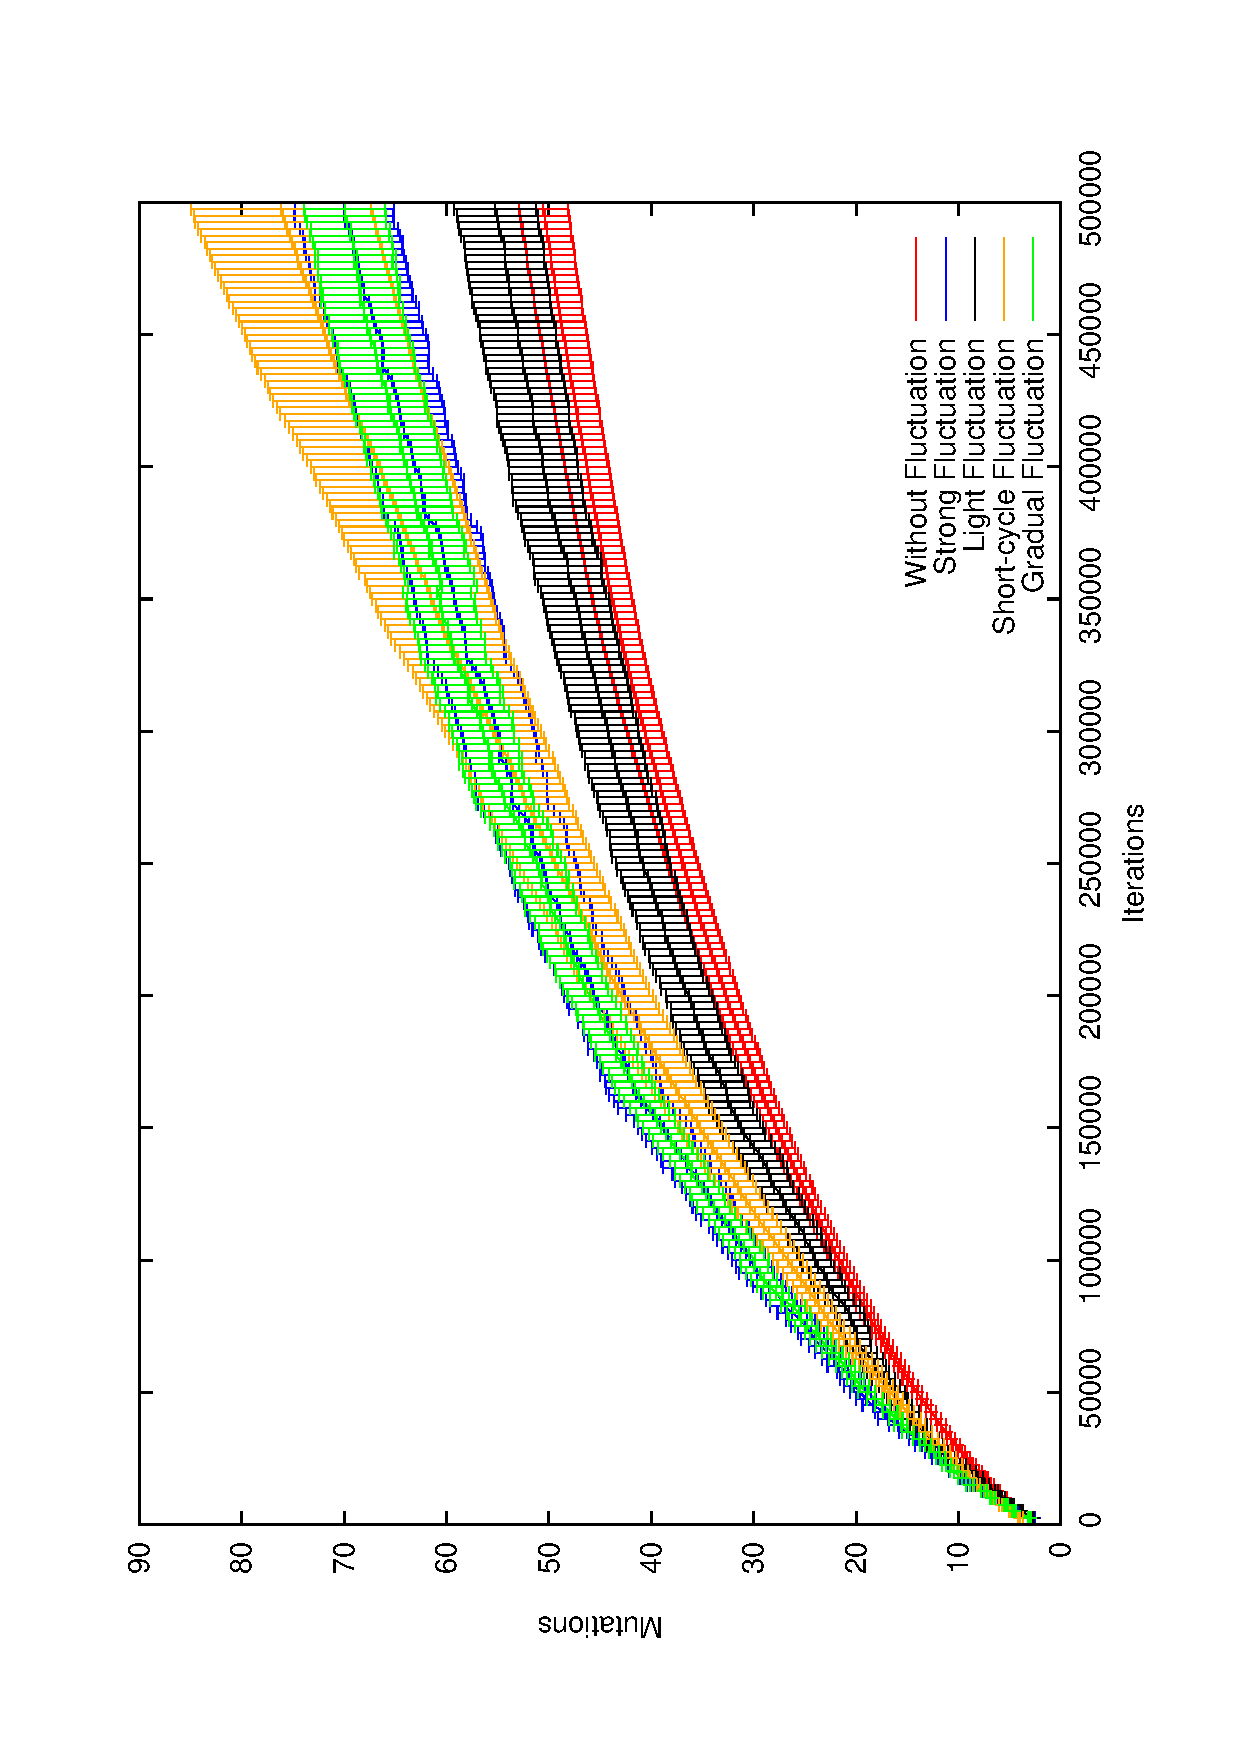
\includegraphics[width=0.7\columnwidth, angle =-90 ]{img/Mutations}
\caption{\textbf{Mutations of genotypes}.
}
\label{fig:Mutations}
\end{figure}

\subsection{Phenotypic Comparison}
Figure~\ref{fig:disimilar} depict phenotypic comparison of disimilar environment, one can see that the impact of environmental fluctuations decreases quickly for \emph{Short-cycle  Fluctuation} while it remains very high for other forms of environmental fluctuations. We also noted that the phenotypic difference of \emph{Short-cycle fluctuations} remains most of the time under the phenotypic differences of the \emph{stable environment}. This suggests a selection of a single phenotype, robust in both environments. Figure~\ref{fig:similar} depict phenotypic comparison of similar environment, it can be observed that, for \emph{Light and Strong fluctuations}, phenotypic differences are much lower than in Figure~\ref{fig:disimilar}, in particular, for \emph{Light fluctuations} they are, most of the time, not significantly different from \emph{stable environment}. The fact that the phenotypic changes induced by environmental fluctuations can be undone by a return to the original environment suggests either plasticity or a strong evolutionary convergence.

\begin{figure}[h]
\centering
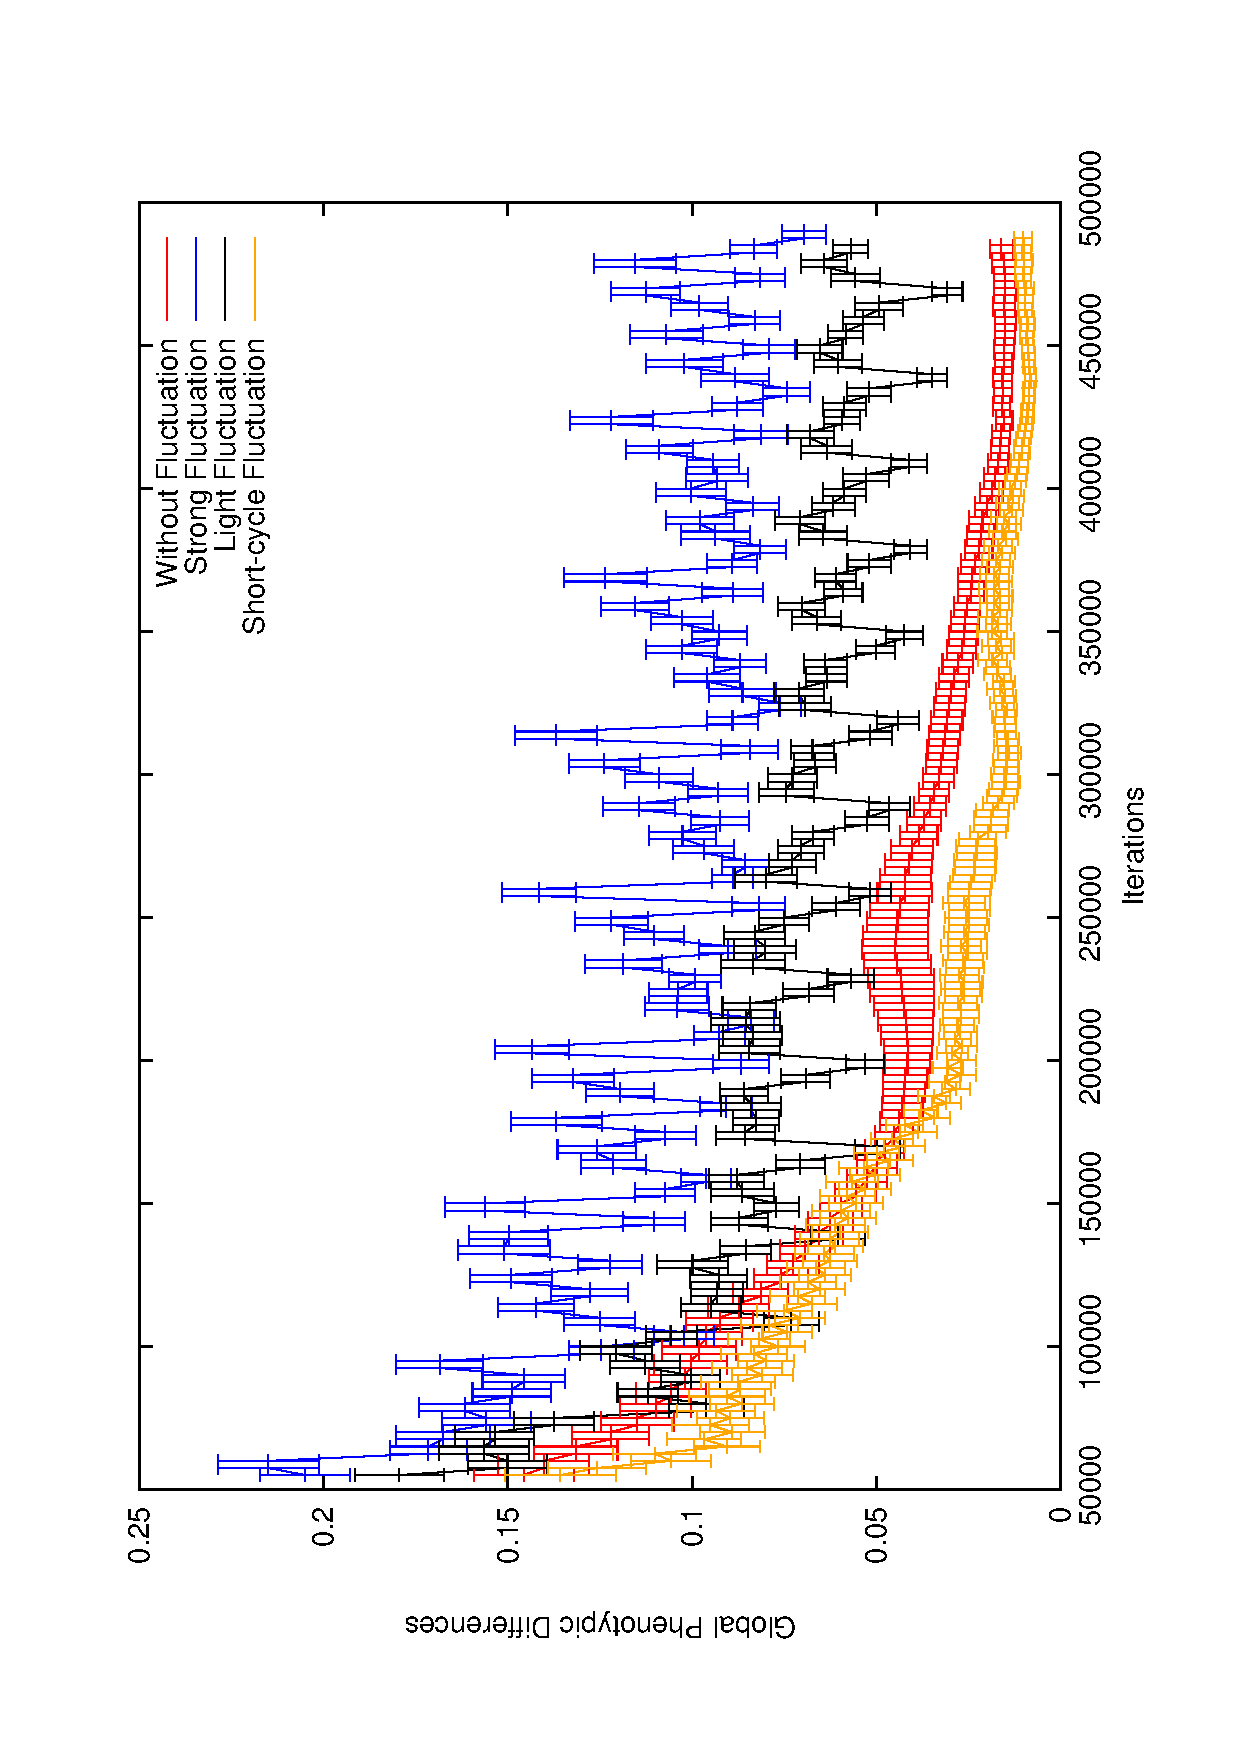
\includegraphics[width=0.7\columnwidth, angle =-90 ]{img/diffProp}
\caption{\textbf{phenotypic comparison of disimilar environments}.}
\label{fig:disimilar}
\end{figure}

\begin{figure}[h]
\centering
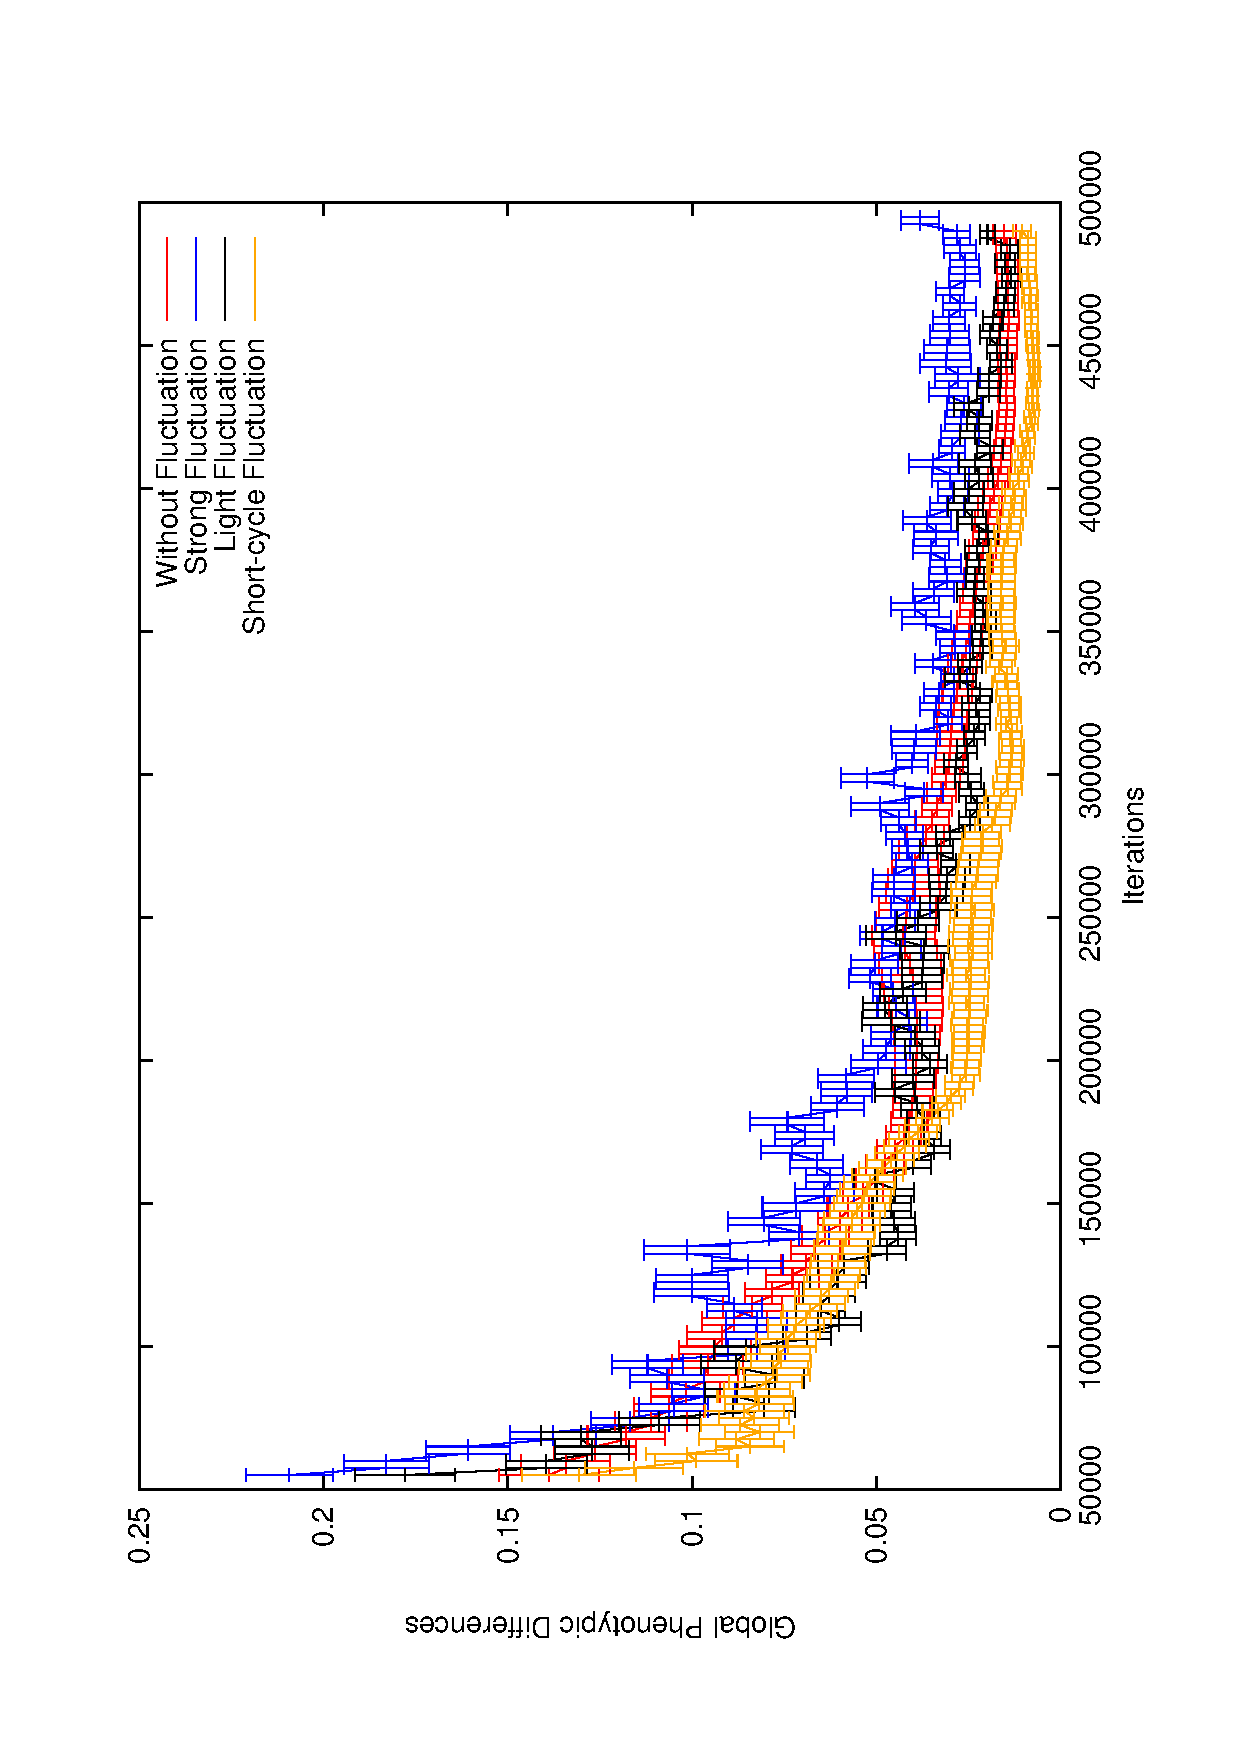
\includegraphics[width=0.7\columnwidth, angle =-90 ]{img/ProgressProp}
\caption{\textbf{phenotypic comparison of similar environments}.}
\label{fig:similar}
\end{figure}




\subsection{Phenotypic and Genotypic Diversity}
Figure \ref{fig:phenodiv} and \ref{fig:genodiv} depict the average phenotypic and genotypic diversities. The low phenotypic diversity of \emph{Short-cycle fluctuations}, suggests the existence in this configuration of a dominant phenotype rather stable over time. While the relatively high phenotypic diversity of \emph{Light and Strong fluctuations} combine with a relatively low genotypic diversity might suggest the existence strong phenotypic selection and therefore some form of plasticity.



\begin{figure}[h]
\centering
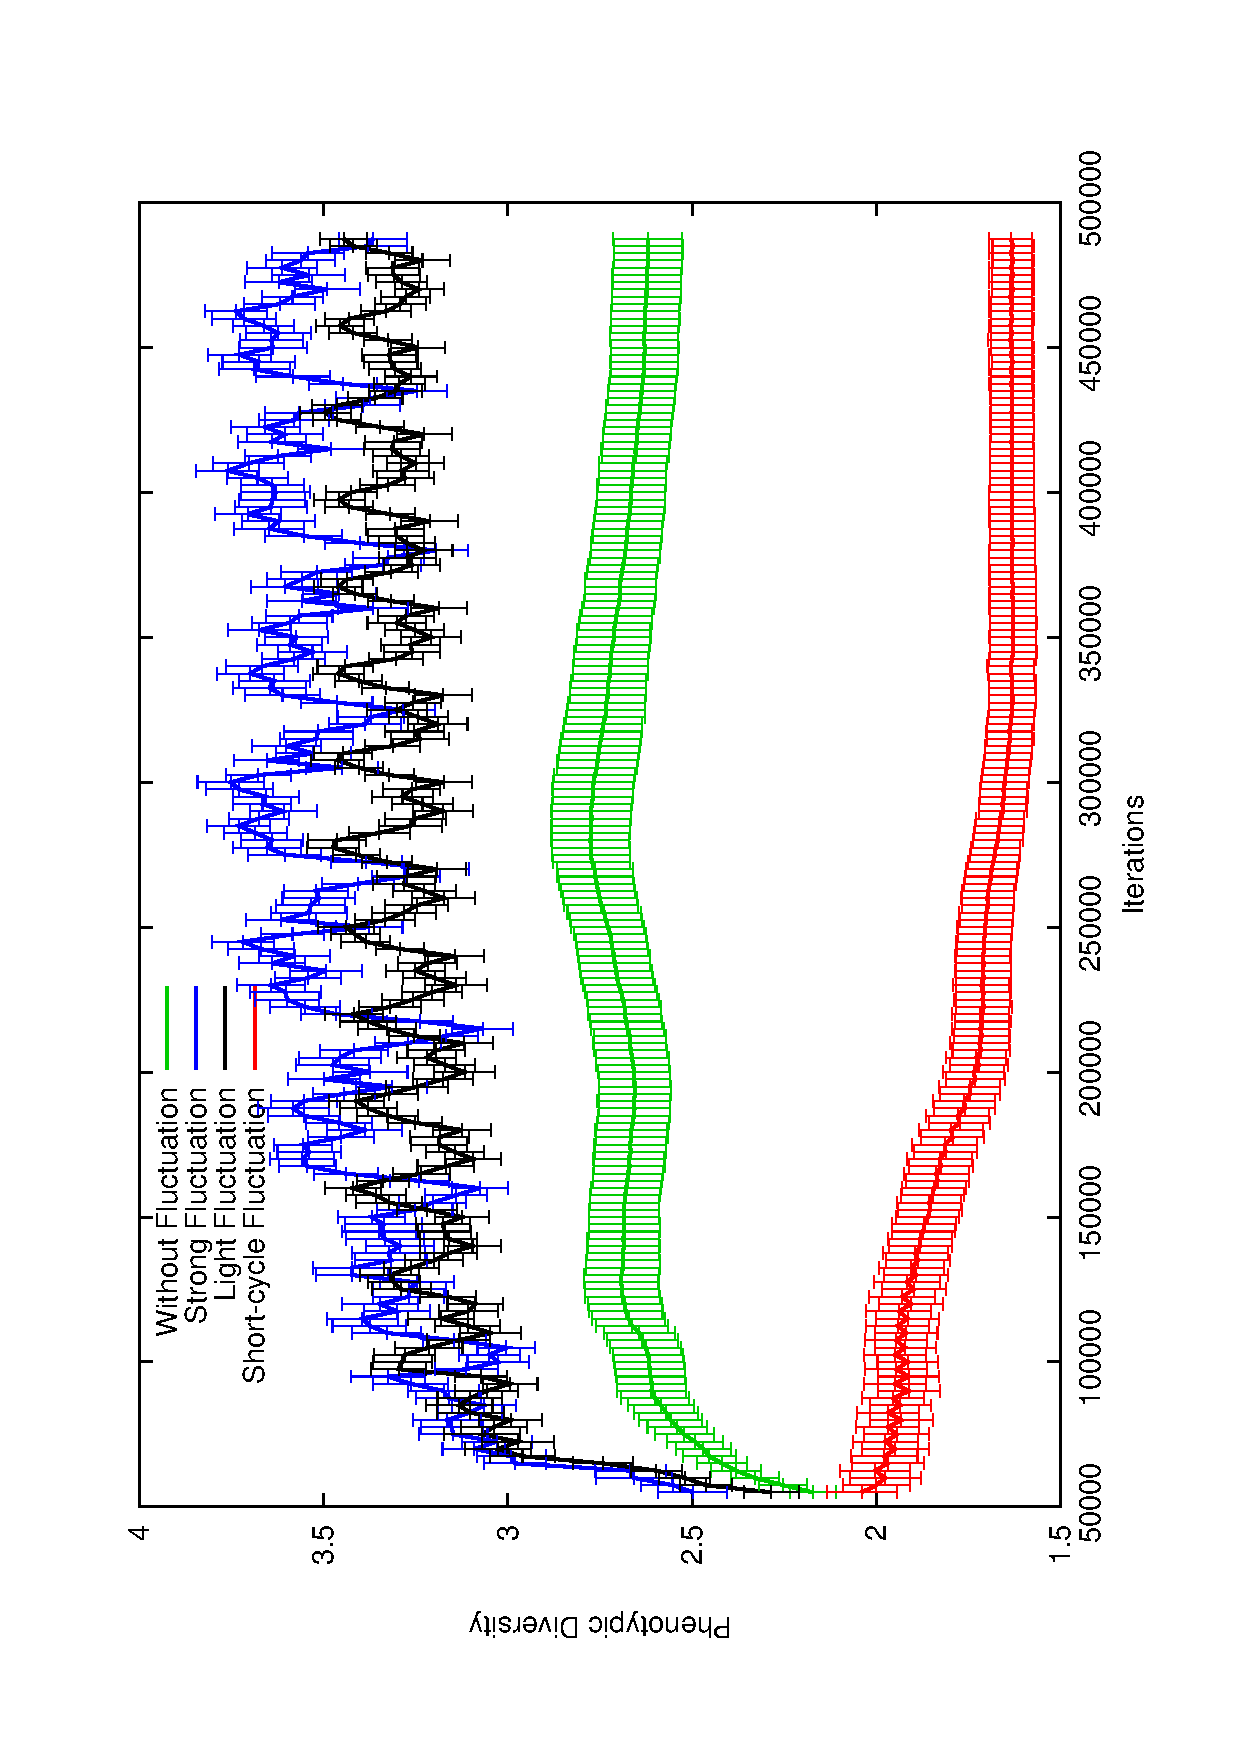
\includegraphics[width=0.7\columnwidth, angle =-90 ]{img/PhenoDiv}
\caption{\textbf{Phenotypic diversity}.}
\label{fig:phenodiv}
\end{figure}

\begin{figure}[h]
\centering
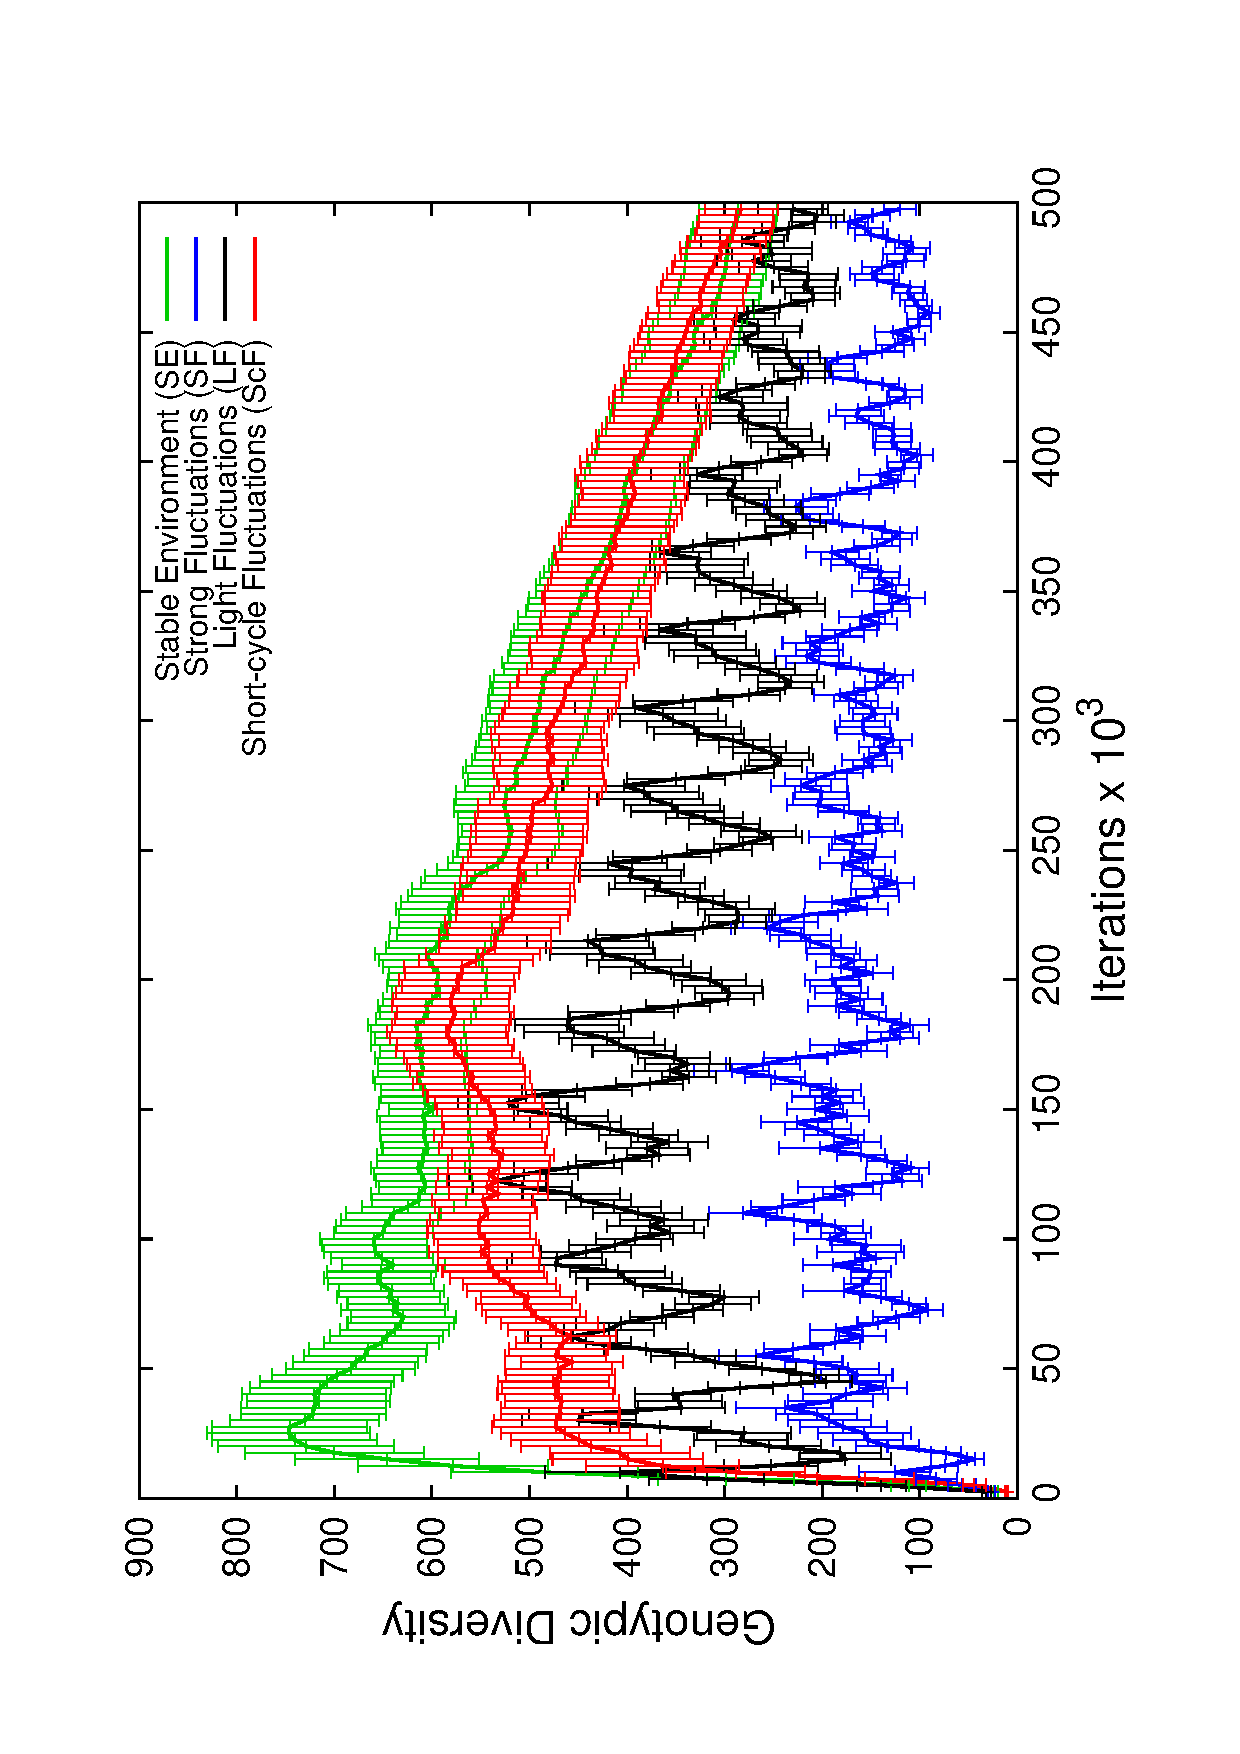
\includegraphics[width=0.7\columnwidth, angle =-90 ]{img/GenoDiv}
\caption{\textbf{Genotypic diversity}.}
\label{fig:genodiv}
\end{figure}

\subsection{Success Rate of Homogenous Test}
Success rates of genotypes in different homogenous simulations are reported in Figure \ref{fig:survrate} using normal approximation interval with a confidence of 95\%. Looking at the different success rates we can first order the different tested environment by increasing difficulty : \emph{Stable Environment}; \emph{Short-cycle Fluctuations}; \emph{Light Fluctuations} ; \emph{Strong Fluctuations}. The fact that the \emph{stable environment} offers the lowest challenge is not surprising. Similarly the fact that \emph{Light Fluctuations} are less difficult than \emph{Strong fluctuations} is quite expected. We believe that the slightest difficulty in \emph{Short-cycle Fluctuations} than in \emph{Light Fluctuations} is due to the reduced number of different environment in \emph{Short-cycle Fluctuations} and, in particular, to the fact that, in this configuration, one of the living state is allowed for all environments $K(S_3)=1$. It is also noteworthy that individuals from \emph{Strong and Light Fluctuations} seem relatively robust in various environmental configurations while those from \emph{Short-cycle Fluctuations} doesn't seem robust outside environmental conditions in which they evolved. Moreover, among genotypes collected from iteration 102500, these same individuals are the only ones that do not reach a 100\% survival ratio in a stable environment.


\begin{figure*}[h]
\centering
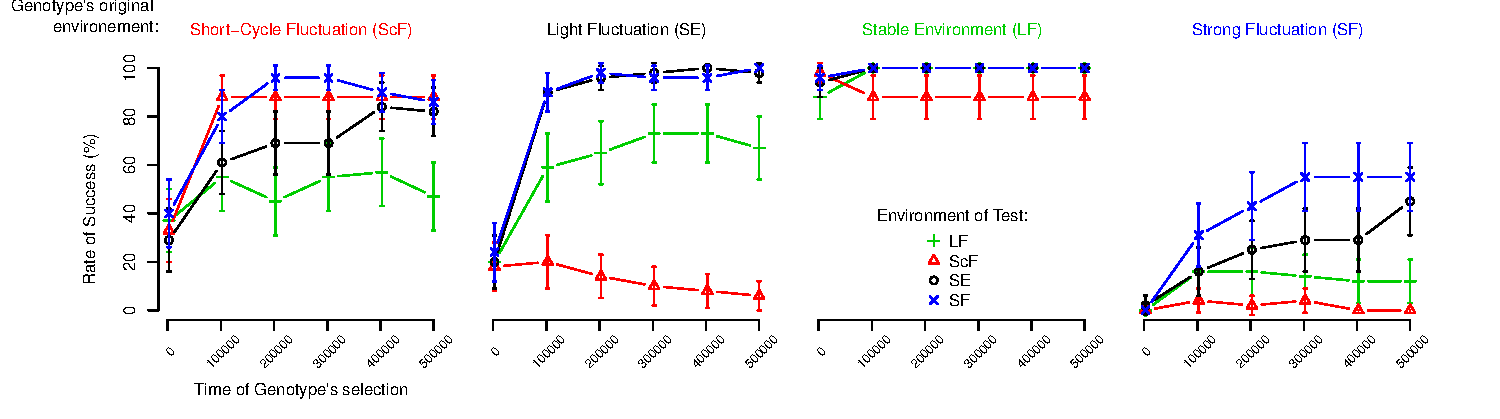
\includegraphics[width=2\columnwidth]{img/testSurvivingRates}
\caption{\textbf{Success Rate of genotypes in Homogenous Tests}.}
\label{fig:survrate}
\end{figure*}

\subsection{Ending Iteration}

Figure \ref{fig:ending} depict the last iteration with living cells of homogenous runs that didn't reach 60000. Note that \emph{Short-cycle Fluctuation} genotypes failures are concentrated around iteration 15000 on \emph{Light Fluctuation} homogenous test and around iteration 25000 on \emph{Strong Fluctuation} homogenous test. This corresponds, for these two configurations, to the first environment for which $K(S_3)=0$, while $K(S_3)=1$ for every environment used in \emph{Short-cycle Fluctuation}. But we also see that some of the genotypes from \emph{Short-cycle Fluctuation} fail during the early iterations of Homogenous test regardless of the used configurations including \emph{Stable Environment} and \emph{Short-cycle Fluctuation}.

This imply that the ecosystem resulting the evolutionary history of individuals plays an key role in their ability to survive. This failure reminds the impossibility of saving species by the unique preservation of their DNA mentioned in \cite{jablonka2014evolution}: \say{You would have to reconstruct the community, and often these communities are very old, with historical memories that are stored in their epigenetic and behavioral systems. These are part of their “identity,” part of their stability. You cannot freeze these memories: they have to be maintained and transmitted through use, so you cannot reconstruct the communities from their component parts.}\emph{(ibid. p. 363)}.

\begin{figure}[H]
\begin{subfigure}{.25\textwidth}
  \centering
  \includegraphics[width=.7\linewidth, angle =-90]{img/boxendingsFailedstable.eps}
  \caption{Stable environment.}
  \label{fig:sfig1}
\end{subfigure}%
\begin{subfigure}{.25\textwidth}
  \centering
  \includegraphics[width=.7\linewidth, angle =-90]{img/boxendingsFailedvariation.eps}
  \caption{Strong Fluctuation.}
  \label{fig:sfig2}
\end{subfigure}

\begin{subfigure}{.25\textwidth}
  \centering
  \includegraphics[width=.7\linewidth, angle =-90]{img/boxendingsFailedvariationLight.eps}
  \caption{Light Fluctuation.}
  \label{fig:sfig2}
\end{subfigure}%
\begin{subfigure}{.25\textwidth}
  \centering
  \includegraphics[width=.7\linewidth, angle =-90]{img/boxendingsFailedvariationSmall.eps}
  \caption{Small Fluctuation.}
  \label{fig:sfig1}
\end{subfigure}
\caption{\textbf{Last iteration with living cells} of homogenous runs that didn't reach 60000 iterations.}
\label{fig:ending}
\end{figure}



%\subsection{Phenotypic Densities}
%Figure \ref{fig:density} depict the density of phenotypes as measured in homogeneous tests. 

%\begin{figure}[H]
%\begin{subfigure}{.25\textwidth}
%  \centering
%  \includegraphics[width=.7\linewidth, angle =-90]{img/boxdensitystable.eps}
%  \caption{Stable environment.}
%  \label{fig:sfig1}
%\end{subfigure}%
%\begin{subfigure}{.25\textwidth}
%  \centering
%  \includegraphics[width=.7\linewidth, angle =-90]{img/boxdensityvariation.eps}
%  \caption{Strong Fluctuation.}
%  \label{fig:sfig2}
%\end{subfigure}

%\begin{subfigure}{.25\textwidth}
%  \centering
%  \includegraphics[width=.7\linewidth, angle =-90]{img/boxdensityvariationLight.eps}
%  \caption{Light Fluctuation.}
%  \label{fig:sfig2}
%\end{subfigure}%
%\begin{subfigure}{.25\textwidth}
%  \centering
%  \includegraphics[width=.7\linewidth, angle =-90]{img/boxdensityvariationSmall.eps}
%  \caption{Small Fluctuation.}
%  \label{fig:sfig1}
%\end{subfigure}
%\caption{Density of Genotype : Each genotype density is processed in four possible different environments.}
%\label{fig:density}
%\end{figure}


